\documentclass[a4paper,12pt]{article} % тип документа

% report, book



%  Русский язык

\usepackage[T2A]{fontenc}			% кодировка
\usepackage[utf8]{inputenc}			% кодировка исходного текста
\usepackage[english,russian]{babel}	% локализация и переносы
\usepackage{graphicx}
\usepackage{tikz}
\graphicspath{{./}}
\DeclareGraphicsExtensions{.png,.jpg}


% Математика
\usepackage{amsmath,amsfonts,amssymb,amsthm,mathtools} 


\usepackage{wasysym}

%Заговолок
\author{Бредихин Александр}
\title{Домашняя работа №1}
\date{}



\begin{document} % начало документа
\maketitle
\newpage

\section*{Matrix calculus}
\subsection*{Задача 1}
Find $\nabla f(x)$, if $f(x) = ||Ax||_2 , x \in \mathbb{R}^p \setminus {0}$.\\
По определению второй нормы: $ f(x)=\sqrt{\langle A x, A x\rangle} $\\
Диффиринцируем, как сложную функция, используя то, что 
$$ \text{(1)  } d \langle x, x \rangle = \langle x, dx \rangle \quad \text{(2)  } \langle y, A x \rangle = \langle A^T y, x \rangle $$ 
получаем: 
$$
d f(x)=\frac{d\langle A x, A x\rangle}{2 \sqrt{\langle A x, A x\rangle}} =(1) \frac{2\langle A x, A d x\rangle}{2 ||A x ||_2}=
$$
$$
= \frac{\langle A x, A d x\rangle}{ ||A x ||_2} = (2) \frac{\langle A^T A x, d x\rangle}{ ||A x ||_2} 
$$
$$
= \langle \frac{ A^T A x} { ||A x ||_2}, d x\rangle
$$
Получаем ответ: $\nabla f(x) = \frac{ A^T A x} { ||A x ||_2}$


\subsection*{Задача 2}
Find $f''(X)$, if $f(X) = \log \det X$

Note: here under $f''(X)$ assumes second order approximation of $f(X)$ using Taylor series: $$ f(X + \Delta X) \approx f(X) + \mathbf{tr}(f'(X)^\top \Delta X) + \frac{1}{2}\mathbf{tr}(\Delta X^\top f''(X) \Delta X) $$

Аналогично, как делали на семинаре получим сначала градиент функции $f(X) = \log \det X$\\
Пусть $ Z \in \mathbf{S}_{++}^{n} $ - близко к $ X $ и $ \Delta X=Z-X $, считаем, что $ \Delta X $ - мала. Сделаем несколько преобразований: 
$$
\begin{aligned}
\log \operatorname{det} Z &=\log \operatorname{det}(X+\Delta X) \\
&=\log \operatorname{det}\left(X^{1 / 2}\left(I+X^{-1 / 2} \Delta X X^{-1 / 2}\right) X^{1 / 2}\right) \\
&=\log \operatorname{det} X+\log \operatorname{det}\left(I+X^{-1 / 2} \Delta X X^{-1 / 2}\right) \\
&=\log \operatorname{det} X+\sum_{i=1}^{n} \log \left(1+\lambda_{i}\right)
\end{aligned}
$$
где $ \lambda_i $ -собственные числа матрицы $ X^{-1 / 2} \Delta X X^{-1 / 2} $. Настал момент использовать, что матрица $ \Delta X $ - очень мала. Из этого следует, что её собственные числа тоже малы и $ \log (1 + \lambda_i) \simeq \lambda_i $ (из ряда Тейлора для скалярных переменных). Получаем, что:
$$
\log \operatorname{det} Z \approx \log \operatorname{det} X+\sum_{i=1}^{n} \lambda_{i}
$$
Теперь пользуясь определением следа (что это как раз есть сумма диагональных элементов, а для матрицы $ X^{-1 / 2} \Delta X X^{-1 / 2} $ сумма собственных значений) и тем, что $ \operatorname{tr}(A B)=\operatorname{tr}(B A) $, получаем: 
$$
\begin{aligned}
\log \operatorname{det} Z & \approx \log \operatorname{det} X+\sum_{i=1}^{n} \lambda_{i} \\
&=\log \operatorname{det} X+\operatorname{tr}\left(X^{-1 / 2} \Delta X X^{-1 / 2}\right) \\
&=\log \operatorname{det} X+\operatorname{tr}\left(X^{-1} \Delta X\right) \\
&=\log \operatorname{det} X+\operatorname{tr}\left(X^{-1}(Z-X)\right)
\end{aligned}
$$
Получается:
$$
f(Z) \approx f(X)+\operatorname{tr}\left(X^{-1}(Z-X)\right)
$$
А значит гдаиент $ f(X) = \log \det X $ записывается как: 
$$
\nabla f(X)=X^{-1}
$$
Теперь аналогичным образом ищем гессиан нашей функции. То есть пусть $ Z \in \mathbf{S}_{++}^{n} $ - близко к $ X $  и $ \Delta X=Z-X $, считаем, что $ \Delta X $ - мала, тогда делая аналогичные преобразования, получаем: 
$$
\begin{aligned}
Z^{-1} &=(X+\Delta X)^{-1} \\
&=\left(X^{1 / 2}\left(I+X^{-1 / 2} \Delta X X^{-1 / 2}\right) X^{1 / 2}\right)^{-1} \\
&=X^{-1 / 2}\left(I+X^{-1 / 2} \Delta X X^{-1 / 2}\right)^{-1} X^{-1 / 2} \\
& \approx X^{-1 / 2}\left(I-X^{-1 / 2} \Delta X X^{-1 / 2}\right) X^{-1 / 2} \\
&=X^{-1}-X^{-1} \Delta X X^{-1}
\end{aligned}
$$

Тут, где написан знак приблежённого равно, как и для вычисления градиента, воспользовался тем фактом, что $ (I+\Delta X)^{-1} \approx I-\Delta X $. \\
Это тензор 4го ранга, поэтому удобно будет записать в виде квадратичной формы от матриц $ M, N $ и представляя в виде следа, то есть $
-\operatorname{tr}\left(X^{-1} M X^{-1} N\right)
$\\
Тогда полное разложение до 2го порядка записывается как: 
$$
\begin{aligned}
f(Z) &=f(X+\Delta X) \\
& \approx f(X)+\operatorname{tr}\left(X^{-1} \Delta X\right)-\frac{1}{2} \operatorname{tr}\left(X^{-1} \Delta X X^{-1} \Delta X\right) \\
& \approx f(X)+\operatorname{tr}\left(X^{-1}(Z-X)\right)-\frac{1}{2} \operatorname{tr}\left(X^{-1}(Z-X) X^{-1}(Z-X)\right)
\end{aligned}
$$



\subsection*{Задача 3}
Calculate the Frobenious norm derivative: $\dfrac{\partial}{\partial X}||X||_F^2$ \\

Из семинара (ну и вообще по свойству нормы Фробениуса) верно, что $ ||X||_F^2 =  \mathbf{tr} \left( X^T X \right) = \mathbf{tr} \left(X X^T \right) = \langle X, X \rangle $, тогда получаем: 
$$
\dfrac{\partial}{\partial X}||X||_F^2 = \dfrac{\partial}{\partial X} \langle X, X \rangle 
$$
По определению производной скалярного произведения, обозначая за $ g = ||X||_F^2 $:
$$
d g = 2 \langle X, d X \rangle
$$
Следовательно, ответ: $ \dfrac{\partial}{\partial X}||X||_F^2 = 2 X $


\subsection*{Задача 4}
Calculate the derivatives of the loss function with respect to parameters $\frac{\partial L}{\partial W}, \frac{\partial L}{\partial b}$ for the single object $x_i$ (or, $n = 1$) 
\begin{figure}[h!]
\begin{minipage}[h]{1\linewidth}
\begin{center}
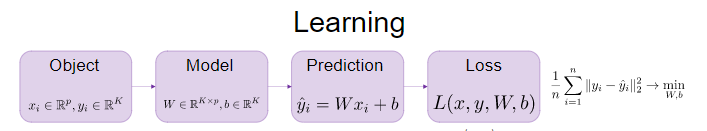
\includegraphics[width=1\linewidth]{shem}
\label{fuuuu} %% метка рисунка для ссылки на него
\end{center}
\end{minipage}
\end{figure} 

(прохожу курс по нейронным сетям и там как раз нужно было писать градиентный спуск для линейной регрессии, так что тут матричное исчесление очень помогло, спасибо!)\\

Так как считаем для одного набора фичей, лосс функция имеет вид: 
$$
L=\|y-\hat{y}\|_{2}^{2}=\|y-\left( Wx +b \right)\|_{2}^{2} = \langle y-\hat{y}, y-\hat{y}\rangle= 
$$
$$
=\langle y-W x-b, y-W x-b\rangle
$$
Теперь берём производную от скалярного произведения сначала по матрице $ W $ затем по вектору $ b $:
$$
\frac{\partial L}{\partial W}=2\left\langle y-Wx-b, \frac{\partial}{\partial W}(y-W x-B)\right\rangle=
$$
$$
= 2 \langle y - \hat{y}, -x d W \rangle = -2 \langle x^T \left( y - \hat{y} \right), d W \rangle
$$
Получается: $ \frac{\partial L}{\partial W} = - 2 x^T \left( y - \hat{y} \right) $\\
Аналогично для производной по вектору $ b $:
$$ \frac{\partial L}{\partial b} = 2 \langle y - \hat{y}, -d b \rangle $$
$$ \Rightarrow \frac{\partial L}{\partial b} = - 2 \left( y - \hat{y} \right) $$
Ответ: 
$$
\frac{\partial L}{\partial W} = - 2 x^T \left( y - \hat{y} \right) \quad \quad \frac{\partial L}{\partial b} = - 2 \left( y - \hat{y} \right)
$$

\newpage
\section*{Projection}
\subsection*{Задача 1}
Find the projection of the matrix $X$ on a set of matrices of rank $k, \quad X \in \mathbb{R}^{m \times n}, k \leq n \leq m$. In Frobenius norm and spectral norm.\\

Формализуем задачу: пусть $ C=\left\{X \in \mathbf{R}^{m \times n} \mid \operatorname{rank} X = k\right\} $,\\ где $
k \leq \min \{m, n\}, \text { и } X_{0} \in \mathbf{R}^{m \times n} $.\\ Представим матрицу $ X_0 $ в сингулярном разложении, то есть $ X_{0}=\sum\limits_{i=1}^{r} \sigma_{i} u_{i} v_{i}^{T} $, где $ r = rank X_0 $, а $  \sigma_i  $ - сингулярные числа. В матричной форме это можно записать как: 
$$
X=U \Sigma V^{T}
$$
где $ U, V $ - ортогональные матрицы, $ \Sigma $ - диагональная с сингулярными числами $ \sigma_1 \geq \sigma_2 \geq \ldots \geq \sigma_n \geq 0 $\\
Ну и как в пацанских задачах на проекцию делаем гипотезу, что матрица $ Y = \pi_{C} \left( X_0 \right) = \sum\limits_{i=1}^{\min\left( k, r \right)} \sigma_{i} u_{i} v_{i}^{T} $ - будет проекцией матрицы $ X_0 $ на множество матриц $ C $. При этом такой ответ будет в обоих нормах.\\

Вообще получили задачу на низкоранговую аппроксимацию: потерять как можно меньше данных о матрице заменив её матрицей меньшим рангом. Начинаем доказывать нашу гипотезу: \\
Если $ \min\left( k, r \right) = r $, то всё понятно и проекция совпадает с самой матрицей.\\ Интересен случай, когда $ r \geq k $. Рассмотрим спектральную норму матрицы:\\
Это норма определяется как максимальное сингулярное число матрицы. Тогда замечаем, что 
$$
\mid \mid \pi_{C} \left( X_0 \right) - X_0 \mid \mid_ 2 = \sigma_{k+1}
$$
Так как просто вычитаем из исходной матрицы матрицу такую же только обрезанную до ранга $ k $. В итоге уходят первые $ k $ сингулярных чисел и максимальное становится $ \sigma_{k+1} $.\\
Теперь хотим показать, что какую матрицу из $ C $ мы не возьмём, а её мы будем представлять, как $
B_{k}=X Y^{\top} \text {где } X \text { и } Y \text { имеют } k \text { колонок }
$ (так как она ранга $ k $), то $$
\left\|\pi_{C} \left( X_0 \right) - X_0\right\|_{2}=\sigma_{k-1} \leq\left\|X_0-B_{k}\right\|_{2}
$$
Ранг искодной матрицы больше, чем $ k $, следовательно, по определению ранга, у матрицы $ V $ должны быть $ k+1 $ линейно независимых столбцов. Составим нетривиальную линейную комбинацию из этих столбцов и назовём полученный вектор $ w $
$$
w=\gamma_{1} v_{1}+\cdots+\gamma_{k+1} v_{k+1}
$$
Без ограничения общности примем, что $
\|w\|_{2}=1 \text { или, что эквивалентно } \gamma_{1}^{2}+\cdots+\gamma_{k+1}^{2}=1
$\\
Так как у матрицы $ Y $ $ k $ линейно независимых столбцов, то $ Y^T w = 0 $. Ну и получаем такое неравенство (зная, что $ B w = 0 $):
$$
\left\|X_0-B_{k}\right\|_{2}^{2} \geq\left\|\left(X_0-B_{k}\right) w\right\|_{2}^{2}=\|X_0 w\|_{2}^{2}=\gamma_{1}^{2} \sigma_{1}^{2}+\cdots+\gamma_{k+1}^{2} \sigma_{k+1}^{2} \geq \sigma_{k+1}^{2}
$$
Получили, что какую матрицу $ B \in C $ не возьмём все равно $ \left\|\pi_{C} \left( X_0 \right) - X_0\right\|_{2}=\sigma_{k-1} \leq\left\|X_0-B_{k}\right\|_{2} $, то есть $ Y $ - проекция $ X_0 $ на $ C $ по определению в спектралной норме. \\

Теперь будем показывать то же самое но уже в Фробениувской норме. Берём ту же гипотезу и также пользуемся сингулярным разложением, только сейчас по определению нормы матрицы: 
$$
\left\| \pi_{C} \left( X_0 \right) - X_0 \right\|_ 2 = \left\| \sum\limits_{i=k+1}^{n} \sigma_{i} u_{i} v_{i}^{T} \right\| = \sum\limits_{i=k+1}^{n} \sigma_{i}^{2}
$$
И снова хотим показать, что какую матрицу $
B_{k}=X Y^{\top} \text {где } X \text { и } Y \text { имеют } k \text { колонок }
$ из $ C $ мы не возьмём, норма разницы исходной матрицы с ней будет больше или равна, чем данная. Ну давайте сделаем это. Для начала воспользуемся знаниями линала:\\
матрицу $ X $ можно представить как $ X=X^{\prime}+X^{\prime \prime} $ и применить неравество треугольника для первых сингулярных чисел, то есть $ \sigma_1 \left( X \right) \leq \sigma_1 \left( X^{\prime} \right) + \sigma_1 \left( X^{\prime\prime} \right) $\\
Аналогичным образом разложим матрицу $ Y = \sum\limits_{i = 1}^k \sigma_i u_i v_i^T $, которая и является нашим кандитатом на проекцию. $ \forall i, j \geq 1 $
$$
\begin{array}{c}
\sigma_{i}\left(Y^{\prime}\right)+\sigma_{j}\left(Y^{\prime \prime}\right)=\sigma_{1}\left(Y^{\prime}-Y_{i-1}^{\prime}\right)+\sigma_{1}\left(Y^{\prime \prime}-Y_{j-1}^{\prime \prime}\right) \geq \\
\geq \sigma_{1}\left(Y-Y_{i-1}^{\prime}-Y_{j-1}^{\prime \prime}\right) \geq \sigma_{1}\left(Y-Y_{i+j-2}\right) \geq \\
\geq \sigma_{i+j-1}(Y)
\end{array}
$$
Предпоследний переход делаем, так как $
R g\left(Y_{i-1}^{\prime}+Y_{j-1}^{\prime \prime}\right) \leq R g\left(Y_{i+j-2}\right)
$\\
Заметим, что так как ранг матрицы $ B_k $ равен $ k $, то $ \sigma_{k+1}(B_k) = 0 $ (следует из сингулярного разложения матрицы $ B_k $). Подставляем в полученно выше неравество: $ Y^{\prime} = X_0 - B_k $, $ Y^{\prime \prime} = B_k $, а $ j = k+1 $, получаем, что 
$$
\begin{array}{c}
\sigma_{i}\left(X_0-B_{k}\right)+\sigma_{k+1}\left(B_{k}\right)>\sigma_{i+k+1-1}(X_0) \\
\sigma_{i}\left(X_0-B_{k}\right) \geq \sigma_{i+k}(X_0)
\end{array}
$$
И наконец-то: 
$$
\left\|X_0-B_{k}\right\|_{F}^{2}=\sum_{i=1}^{n} \sigma_{i}\left(X_0-B_{k}\right)^{2} \geq \sum_{i=k+1}^{n} \sigma_{i}(X_0)^{2}=\mid X_0-Y_{k} \|_{F}^{2}
$$
И получили то, что нужно)))

\subsection*{Задача 2}
Prove that projection is a nonexpansive operator, i.e. prove, that if $S \in \mathbb{R}^{n}$ is nonempty, closed and convex set, then for any $(x_{1}, x_{2}) \in \mathbb{R}^{n} \times \mathbb{R}^{n}$

$$ \lVert \pi_{S}(x_{2}) - \pi_{S}(x_{1}) \rVert_{2} \leq \lVert x_{2} - x_{1} \rVert_{2} $$


Покажем, что проекция на замкнутое выпуклое множество - нерасширяющийся оператор, то есть $ \forall x_1, x_2 \in \mathbf{R}$
$$
\left\|\pi_{S}\left(x_{2}\right)-\pi_{S}\left(x_{1}\right)\right\|_{2} \leq\left\|x_{2}-x_{1}\right\|_{2}
$$
Переобозначим, проекцию как: $ \pi_{S}\left(x\right) \equiv P(z) $ (так легче вбивать в тех и в таких обозначениях решал в тетрадке). То есть хотим показать, что 
$$
\left\|P\left(z_{1}\right)-P\left(z_{2}\right)\right\|\leq\left\|z_{1}-z_{2}\right\|
$$
Из семинара свойство проекции на замкнутое выпуклое множество - $ S $ звучит как: $ \forall x \in S $
$$
\langle P(z_1) - z_1, x - P(z_1) \rangle \geqslant 0 \Leftrightarrow \langle z_1 - P(z_1) , x - P(z_1) \rangle \leqslant 0
$$
Возьмём вместо $ x $ - $ P(z_2) $ (можем так сделать, так как $ \forall x \in S $ и $ P(z_2) \in S $ по определению проекции). Тогда получим такое неравенство: 
$$
\langle z_1 - P(z_1) , P(z_2) - P(z_1) \rangle \leqslant 0
$$
Аналогично запишем неравенство  (те же самы рассуждения только начнём с проекции для второй точки)
$$
\langle z_2 - P(z_2) , P(z_1) - P(z_2) \rangle \leqslant 0 \Leftrightarrow \langle P(z_2) - z_2 , P(z_2) - P(z_1) \rangle \leqslant 0
$$
А теперь сложим два полученных неравенства и немного преобразуем их: 
$$
\langle z_1 - P(z_1) , P(z_2) - P(z_1) \rangle + \langle P(z_2) - z_2 , P(z_2) - P(z_1) \rangle \leqslant 0
$$
$$
\langle z_1 - z_2 + P(z_2) - P(z_1), P(z_2) - P(z_1) \rangle \leqslant 0
$$
$$
\Rightarrow \langle P(z_2) - P(z_1), P(z_2) - P(z_1) \rangle \leqslant \langle z_2 - z_1, P(z_2) - P(z_1) \rangle
$$
Для правой части используем любимое неравенство Коши-Буняковского (в этом дз оно ещё пригодитя в разных формах), получаем: 
$$
\Rightarrow \langle P(z_2) - P(z_1), P(z_2) - P(z_1) \rangle \leqslant \langle z_2 - z_1, P(z_2) - P(z_1) \rangle \leqslant \left\| z_2 - z_1 \right\|_{2} \left\| P(z_2) - P(z_1) \right\|_{2}
$$
Заменяя скалярное произведение двух одинаковых элементов их нормой в квадрате, получим: 
$$
\left(\left\| P(z_2) - P(z_1) \right\|_{2} \right)^2 \leqslant \left\| z_2 - z_1 \right\|_{2}  \left\| P(z_2) - P(z_1) \right\|_{2} 
$$
Теперь сокращаем левую и правую часть (так как норма положителльное число, то неравенство не поменяется) и получим:
$$
\left\| P(z_2) - P(z_1) \right\|_{2} \leqslant \left\| z_2 - z_1 \right\|_{2}
$$
Ура! Это то что нам нужно. Значит, мы доказали, что проекция это нерасширяющийся оператор.

\newpage
\section*{Convex sets}
\subsection*{Задача 1}
Prove that if the set is convex, its interior is also convex. Is the opposite true?\\

Сразу скажем, что обратное неверно. Контрпример придумывается легко (пример из семинара):
\begin{figure}[h!]
\begin{minipage}[h]{1\linewidth}
\begin{center}

\includegraphics[width=0.3\linewidth]{not_bro}
\end{center}
\end{minipage}
\end{figure}
Квадратик, внутренность у него выпуклое множество (так как если соединим любые две точки из внутренности, то лининия, соединяющая, их будет полностью принадлежать внутренности). Но само множество невыпуклое, так как если проведём лининию через границу, то она в некоторых местах будет проходить не через точки множества, а, следовательно, множество невыпуклое.\\
Есть пример ещё проще. Возьмём 2 точки на плоскости далеко друг от друга. Их внутренность - пустое множество (по определению внутренности). А пустое множество - выпуклое. Но, конечно, если мы их соеденим линией, то точки линии не принадлежат множеству, следовательно оно само невыпуклое.\\

Теперь докажем, что если множество выпуклое - то его внутренность тоже выпуклое множество.\\

Начнём с тривиального случая: если $ \mathbf{int} (S) = \varnothing $, то оно выпуклое по определению и доказывать ничего не надо.\\

Теперь рассмотрим, когда $ \mathbf{int} (S) \neq \varnothing $. Ну тогда будут существовать точки $ x_1, x_2 \in \mathbf{int} (S) $. По определению внутренности, они также будут принадлежать и $ S $. А $ S $ выпуклое, следовательно прямая соединяющая эти точки лежит в $ S $, но! мб найтись такая точка $ x^* \in \theta x_1 + (1 - \theta) x_2 $, что она не лежит во $ \mathbf{int} (S) $. Так вот сейчас покажем, что такой точки не найдётся, следовательно, все точки на этой прямой - принадлежат внутренности $ S $ и по определению внутренность тоже будет выпуклым множеством.\\

Так как $ x_1, x_2 \in \mathbf{int} (S) $, то по определению внутренности существует шары, каких-то радиусов $ r_1 $ и $ r_2 $, в которых есть другие точки внутренности множества.\\
Будем брать точки, которые лежат на перпендикулярах к проведённой прямой. Эти точки также соединяем прямыми и так как $ S $ - выпуклое множество, то все точки этих прямых будут содержаться в $ S $. Но таким образом мы сможем настроить бесконечно много точек со всех сторон из $ S $ возле точки $ x^* $. Но тогда $ x^* $ по определению уже будет являться внутренней точкой. (картинка для понимания рассуждений)

\begin{figure}[h!]
\begin{minipage}[h]{1\linewidth}
\begin{center}
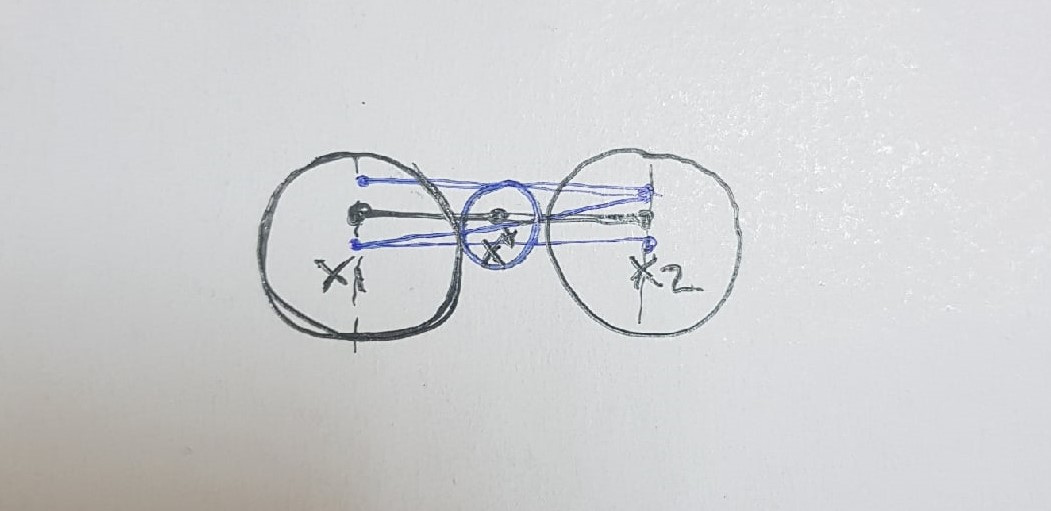
\includegraphics[width=0.6\linewidth]{balls}
\end{center}
\end{minipage}
\end{figure}
Получили, что все точки на прямой соединяющей две точки $ x_1, x_2 \in \mathbf{int} (S) $ тоже принадлежат внутренности, следовательно $ \mathbf{int} (S) $ - выпуклое множество.


\subsection*{Задача 2}
Нужно доказать, что квадратичные, симметричные положительно определённые матрицы образуют выпуклое множество (обозначим его за $ \mathbf{S}_{+}^{n} $).\\

Докажем, что это множество - выпуклый конус. Проверим это по определению: \\
$ \forall \theta_1, \theta_2 \geqslant 0$ и $ \forall A, B \in \mathbf{S}_{+}^{n} $ хотим показать, что 
$
\theta_{1} A+\theta_{2} B \in \mathbf{S}_{+}^{n}
$
Понятно, что матрица, которая получена с помощью такой линейной комбинацией остаётся квадратной и симметричной (симметричной, так как сумма одинаковых чисел, домноженных на одинаковые константы будет одинаковым числом).\\ 
Покажем, что она положительно определена: по определению $ \forall x \in \mathbf{R}^n $
$$
x^{T}\left(\theta_{1} A+\theta_{2} B\right) x=\theta_{1} x^{T} A x+\theta_{2} x^{T} B x \geq 0
$$
так как $
A \succeq 0 \rightarrow x^{T} A x \geqslant 0, B \succeq 0 \rightarrow x^{T} B x \geqslant 0  \text { и } \theta_{1}, \theta_{2} \geq 0
$\\
Показали, что выполнено определение выпуклого конуса. Следовательно, $ \mathbf{S}_{+}^{n} $ - выпуклое.


\subsection*{Задача 3}
Show that the hyperbolic set of $ {x \in \mathbb{R}^n_+ | \prod\limits_{i=1}^n x_i \geq 1 } $ is convex.\\ Hint: For $0 \leq \theta \leq 1$ it is valid, that $a^\theta b^{1 - \theta} \leq \theta a + (1-\theta)b$ with non-negative $a,b$.\\

Ну раз дали подсказку, то используем её)\\
Возьмём $ a = \prod\limits_{i} x_{i} \geq 1 \text { и } b = \prod\limits_{i} y_{i} \geq 1 $ (следовательно $ a,b $ принадлежат нашему множеству по его определению)\\
Подставляем в неравенство, получаем: 
$$
\prod\limits_{i}\left(\theta x_{i}+(1-\theta) y_{i}\right) = \theta \prod\limits_i x_i + \left( 1 - \theta \right) \prod\limits_i y_i  \geq \prod\limits_i x_{i}^{\theta} y_{i}^{1-\theta}=\left(\prod\limits_{i} x_{i}\right)^{\theta}\left(\prod\limits_{i} y_{i}\right)^{1-\theta} \geq 1
$$
Следовательно, по определению выпуклого множества, что для $0 \leq \theta \leq 1$ и $ \forall a, b \in S $, где $ S $ наше множество, выполнено, что $ \theta a + (1 - \theta) b \in S $ (так как получили, что это выражение тоже больше или равно 1)\\
Доказали.


\subsection*{Задача 4}
Prove, that the set $S \subseteq \mathbb{R}^n$ is convex if and only if $(\alpha + \beta)S = \alpha S + \beta S$ for all non-negative $\alpha$ and $\beta$\\

Для начала докажем, что если выполняется, что $(\alpha + \beta)S = \alpha S + \beta S$, то множество $ S $ выпуклое.\\
Доказывать будем по определению, то есть, что $ \forall x_1, x_2 \in S $ и $ \forall \theta \in [0,1] $ выполнено, что $ \theta x_1 + (1 - \theta) x_2 \in S$\\
Используем, что есть, а именно, что $ \forall x \in \alpha S + \beta S$. Верно, что он представляется как: \\
$ x = \alpha z_1 + \beta z_2 $, где $ z_1 \in S \text{и } z_2 \in S$ \\
$ x = (\alpha + \beta) z_3$, где $ z_3 \in S $ (так как $(\alpha + \beta)S = \alpha S + \beta S$)\\
Вынесем скобочку $ \alpha + \beta $ из первого представления. Получим:\\
$$ x = \left( \alpha + \beta \right) \left( \frac{\alpha}{\alpha + \beta} z_1 + \frac{\beta}{\alpha + \beta} z_2 \right) \in S $$
Мы получили вид как во втором представлении, то есть $ z_3 = \frac{\alpha}{\alpha + \beta} z_1 + \frac{\beta}{\alpha + \beta} z_2  \in S $\\
Заметим, что $ \frac{\alpha}{\alpha + \beta} + \frac{\beta}{\alpha + \beta} = 1$.\\
Пусть $ \theta =  \frac{\alpha}{\alpha + \beta} \Rightarrow  \frac{\beta}{\alpha + \beta} = 1 - \theta$, следовательно:\\
$ z_3 = \theta z_1 + (1 - \theta) z_2  \in S $
Так как $(\alpha + \beta)S = \alpha S + \beta S$ верно для произвольных неотрицательных $ \alpha $ и $ \beta $, то $ \theta = \frac{\alpha}{\alpha + \beta} \in [0,1] $. Получили определение выпуклого множества, то есть доказали в одну сторону. Теперь доказываем в обратную.\\

Пусть $ S $ - выпуклое множество, нужно доказать, что $ (\alpha + \beta)S = \alpha S + \beta S $. Это равенство множеств, следовательно, чтобы его доказать, нужно показать 2 включения: 
\begin{itemize}
\item[1) ] $ (\alpha + \beta)S \subseteq \alpha S + \beta S $\\
Возьмём $ z \in (\alpha + \beta)S $, то есть он представим в виде: $ z = (\alpha + \beta)x = \alpha x + \beta x $, где $ x \in S $. Таким образом показали, что любой элемент $ z \in S $ представим как $ z = \alpha x + \beta x $. Это и есть наше включение: $ (\alpha + \beta)S \subseteq \alpha S + \beta S $
\item[2) ] $ \alpha S + \beta S \subseteq (\alpha + \beta)S $\\
Теперь хотим показать, что элемент $ z \in \alpha S + \beta S $, то есть который можно представить как: $ z = \alpha z_1 + \beta z_2 $, где $ z_1, z_2 \in S $, также может быть записан, как $ z = (\alpha + \beta) z_3 $, где $ z_3 \in S $. \\
Как и в доказательстве в другую сторону вынесем скобку $ (\alpha + \beta) $. Получим:\\
$$ z = \left( \alpha + \beta \right) \left( \frac{\alpha}{\alpha + \beta} z_1 + \frac{\beta}{\alpha + \beta} z_2 \right) $$
Снова берём $ \theta = \frac{\alpha}{\alpha + \beta} \Rightarrow \frac{\beta}{\alpha + \beta} = 1 - \theta$. Следовательно:\\
$z = \left( \alpha + \beta \right) \left( \theta z_1 + (1 - \theta) z_2 \right) $\\
Вспоминаем, что $ S $ - выпуклое множество, значит $ \left( \theta z_1 + (1 - \theta) z_2 \right) = z_3 \in S, \forall \theta $\\
А это значит, что $ z = \left( \alpha + \beta \right) z_3 \in S $, то есть мы показали обратное включение.\\

\end{itemize}
Показав оба включения, доказали, что $ S \text{-выпуклая} \Rightarrow (\alpha + \beta)S = \alpha S + \beta S$ и тем самым закончили доказательство задачи.



\subsection*{Задача 5}
Let $x \in \mathbb{R}$ is a random variable with a given probability distribution of $\mathbb{P}(x = a_i) = p_i$, where $i = 1, \ldots, n$, and $a_1 < \ldots < a_n$. It is said that the probability vector of outcomes of $p \in \mathbb{R}^n$ belongs to the probabilistic simplex, i.e. $P = { p \mid \mathbf{1}^Tp = 1, p \succeq 0 } = { p \mid p_1 + \ldots + p_n = 1, p_i \ge 0 }$. Determine if the following sets of $p$ are convex:

\begin{itemize}
\item[1) ] $ \mathbb{P}(x > \alpha) \le \beta $\\
В семинаре в аналогичной задаче мы показали, что можем сводить к ограничениям на $ p $, как ограничения на полупространство. А такое множество выпуклое и мы решили задачу. В первых трёх пунктах будем делать также.\\
Начинаем!!\\
Условие, что $ \mathbb{P}(x > \alpha)  $ по определению можем записать как:  $ \mathbb{P}(x > \alpha) = \sum\limits_{i: a_i \geqslant \alpha} p_i$, следовательно 
$$
\mathbb{P}(x > \alpha) \le \beta \Leftrightarrow \sum\limits_{i: a_i \geqslant \alpha_i} p_i \le \beta
$$
А геометрически это и есть полупространство и оно выпуклое, значит, наше множество тоже выпуклое.\\
Ответ: выпуклое
\item[2) ] $ \mathbb{E} \vert x^{201}\vert \le \alpha \mathbb{E}\vert x \vert $
По определению матожидания (и переносим всё в одну часть): 
$$
\sum\limits_{i=1}^{n} p_{i}\left(\left|a_{i}^{201}\right|-\alpha\left|a_{i}\right|\right) \leq 0
$$
Но нас-то уже не подловить и без разницы какой коэффициент (хоть в 1001 степени $ x $). Главное, чтобы относительно $ p $ было линейное выражение, а у нас оно и получается (можно переписать как $ \sum\limits_{i=1}^{n} c_i p_{i}  $, где $ c_i = \left(\left|a_{i}^{201}\right|-\alpha\left|a_{i}\right|\right) $ - некоторые числовые коэффициенты). Значит, геометрически оно задаёт полупростронство, а оно выпуклое.\\
Ответ: выпуклое
\item[3) ] $ \mathbb{E} \vert x^{2}\vert \ge \alpha  $\\
Перепишем это, воспользовавшийся определением матожидания, получаем: 
$$ \sum\limits_{i} p_i a_i^2 \geqslant \alpha$$
Ну снова то же самое) крч, ответ уже понятен.\\
Ответ: выпуклое
\item[4) ] $ \mathbb{V}x \ge \alpha $
По определению дисперсии и разрядив знания линала получаем: 
$$
\mathbb{V}x = \mathbb{E} x^2 - \left( \mathbb{E} x \right)^2 = \sum_{i=1}^{n} a_{i}^{2} p_{i}-\left(\sum_{i=1}^{n} a_{i} p_{i}\right)^{2}=b^{T} p-p^{T} A p \geqslant \alpha
$$
где $ b_{i}=a_{i}^{2} \text { и } A=a a^{T} $. То есть $ A $ - положительно определённая матрица. Заметим, что такое выражение геометрически задаёт параболу , ветви которой направлены вниз и гиперплоскость $ \alpha $. В нашем множестве лежат точки, которыые как раз ограничиваются этой гиперплоскостью (заштрихованное множество на картинке)
\begin{figure}[h!]
\begin{minipage}[h]{1\linewidth}
\begin{center}
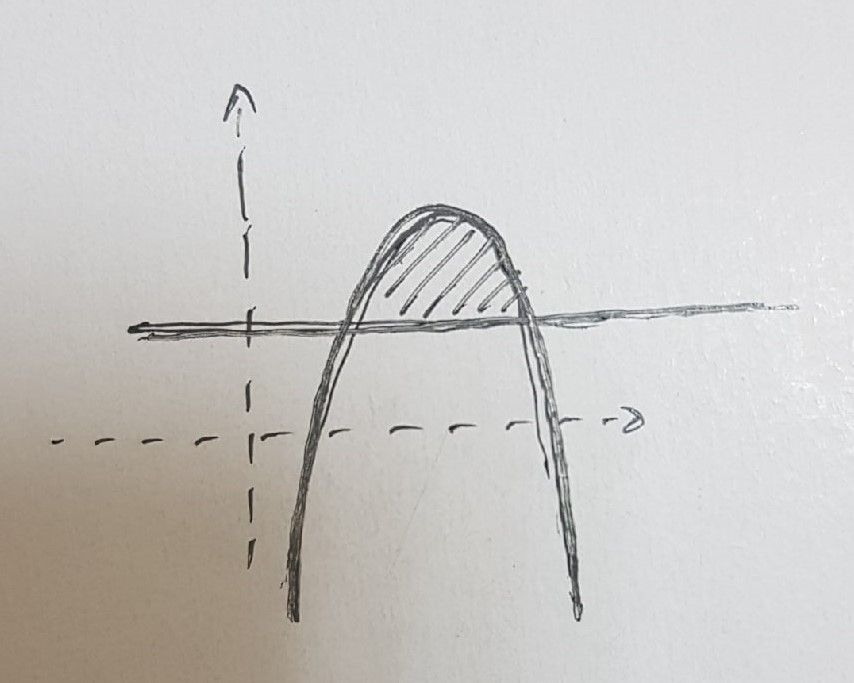
\includegraphics[width=0.5\linewidth]{parab}
\label{fuuuu} %% метка рисунка для ссылки на него
\end{center}
\end{minipage}
\end{figure}
\end{itemize}
А такое множество выпуклое, так как перевёрнутая парабола - вогнутая функция, следовательно, её подграфик - выпуклое множество и мы пересекаем его с гиперплоскостью, то есть множество сохраняет выпуклость. \\

На последнем семинаре вы сказали, что можно доказать строго по определению, но у меня не получилось этого сделать, поэтому оставил такие рассуждения, но не уверен, что это верно. 

\newpage

\section*{Convex functions}
\subsection*{Задача 1}
Prove, that function $f(X) = \mathbf{tr}(X^{-1}), X \in S^n_{++}$ is convex, while $g(X) = (\det X)^{1/n}, X \in S^n_{++}$ is concave.\\


Сначала докажем второй факт, что $ g(x) $ - вогнутая.\\
Видим, что функций возвращает скаляр, следовательно, используем метод "Reduction to a line" (не знаю, как правильно его перевести на русский). Но он заключается в том, что мы представляем нашу функцию $ g(x) $, как:
$$
g(t)=f(Z+t V), \text { где } Z \succ 0 \text { и } V \in \mathbf{S}^{n} \text{обе симметричные}
$$
И теперь рассматриваем её, как функцию от скалярной переменной $ t $, которая принимает значения такие что $\{t \mid Z+t V \succ 0\}$. Делаем все те же преобразования, что и в скрине, который вы скинули в дискорд, получаем: 
$$
\begin{aligned}
g(t) &=(\operatorname{det}(Z+t V))^{1 / n} \\
&=\left(\operatorname{det} Z^{1 / 2} \operatorname{det}\left(I+t Z^{-1 / 2} V Z^{-1 / 2}\right) \operatorname{det} Z^{1 / 2}\right)^{1 / n} \\
&=(\operatorname{det} Z)^{1 / n}\left(\prod_{i=1}^{n}\left(1+t \lambda_{i}\right)\right)^{1 / n}
\end{aligned}
$$
Где $ \lambda_i $ - собственные числа матрицы $ Z^{-1 / 2} V Z^{-1 / 2} $.\\
Из последнего равенства видим, что наша функция $ g(t) $ - вогнута на множестве $\{t \mid Z+t V \succ 0\}$, так как $ \operatorname{det} Z > 0 $, так как $ Z \succ 0 $, и геометрическое среднее $\prod\limits_{i=1}^{n}\left(x_{i}\right)^{1 / n}$ - вогнуто (докажу в 4ой задаче). $ 1 + t \lambda_{i} $ - вогнутая функция, так как линейная.\\
Следовательно, $ g(X) $ - вогнуто.\\


%------------------------------------
Для $f(X) = \mathbf{tr}(X^{-1}), X \in S^n_{++}$\\
Тем же приёмом покажем, что она выпуклая. Рассмотрим $ S (t) = Z + t V $, где $ Z \in S^n_{++} $ и $ V $ - симметрична. Теперь рассматриваем функцию от скалярной переменной $ t $.\\
Достаточно показать (по дифференциальному критерию второго порядка), что 
$$  \dfrac {d ^ 2} {dt ^ 2} \mathbf{tr} (S (t) ^ {- 1}) |_{t = 0} \ge 0 $$
Теперь сделаем матричное разложение в ряд Тейлора в $t = 0$ (так как дифференциал без ограничения общности, мы считаем в этой точке)
$$ S (t) ^ {- 1} = (Z (I + t Z ^ {- 1} V)) ^ {- 1} = Z ^ {- 1} - t Z ^ {- 1} VZ ^ { -1} + t ^ 2 Z^ {- 1} VZ ^ {- 1} VZ ^ {- 1} + \ldots $$ 
поэтому 
$$ \left. \dfrac {d ^ 2} {\partial t ^ 2} \mathbf{tr} (S (t) ^ {- 1}) \right| _ {t = 0} = 2 \mathbf{tr} (Z ^ { -1} VZ ^ {- 1} VZ ^ {- 1}) $$
Но $ Z ^ {- 1} VZ ^ {- 1} VZ ^ {- 1} = CZ ^ {- 1} C ^ T $, где $ C = Z ^ {- 1} V $ и $ Z ^ {- 1 } $ положительно определены (так как $ Z \in S^n_{++} $ и  $ V $ - симметрична),\\ поэтому $ CZ ^ {- 1} C ^ T $ положительно полуопределена,\\ поэтому $ \mathbf{tr} (CZ ^ {- 1} C ^ T) \ge 0 $.\\
Следовательно, $f(X) = \mathbf{tr}(X^{-1})$ - выпуклая функция.
%-----------------------------------------



\subsection*{Задача 6}
Is $f(x) = -x \ln x - (1-x) \ln (1-x)$ convex?\\


Логичнее решить эту задачу здесь, так как это известная функция кросс-энтропии, которую уже юзал для классификации и градиентный спуск сошёлся, поэтому скорее всего с ней всё хорошо и она выпуклая, посмотрим так ли это?) (а также, ответив на этот вопрос, сможем решить 2ую задачу)\\

Рассмотрим отдельно $ f(x) = x \ln x $, где $ x $ - скалярная переменная и покажем по дифференциальному критерию второго порядка, что она выпуклая. Действительно: 
$$
f^{\prime}(x)=\ln x+1, \quad f^{\prime \prime}(x)=1 / x
$$
Так как $ x $ стоит под логарифмом, то $ x > 0 $, следовательно, $ f^{\prime \prime}(x) > 0 $. Значит $ f(x) = x \ln x $ строго выпуклая функция. \\

Значит, функция $ g(x) = (1 - x) \ln (1 - x) $ тоже строго выпуклая при $ 1 - x > 0 $. При классификации это условие выполнено, так как кросс-энтропии мы подаём значения после софтмакска, который возвращает вектор, где каждое число $ 0 < x_i < 1 $ (вероятности принадлежности к каждому классу).\\

Неотрицательная сумма выпуклых функций сохраняет выпуклость, поэтому $ x \ln x + (1 - x) \ln (1 - x) $ - строго выпуклая функция. Но у нас в задании она стоит с минусом, значит, вогнутая по определению.\\
Ответ: вогнутая

\subsection*{Задача 2}
Kullback–Leibler divergence between $p,q \in \mathbb{R}^n_{++}$ is:

$$ D(p,q) = \sum\limits_{i=1}^n (p_i \log(p_i/q_i) - p_i + q_i) $$

Prove, that $D(p,q) \geq 0 \forall p,q \in \mathbb{R}^n_{++}$ and $D(p,q) = 0 \leftrightarrow p = q$

Hint: $ D(p,q) = f(p) - f(q) - \nabla f(q)^T(p-q), \quad f(p) = \sum\limits_{i=1}^n p_i \log p_i $


Проверим подсказку, которая дана в условии задачи. По определению дивергенция Кульбака-Лейблера:
$$
D(p, q)=\sum_{i=1}^{n}\left(p_{i} \log \left(p_{i} / q_{i}\right)-p_{i}+q_{i}\right)
$$
И мы замечаем, что оно равно 
$$
D(p, q)=f(p)-f(q)-\nabla f(q)^{T}(p-q), \quad f(p)=\sum_{i=1}^{n} p_{i} \log p_{i}
$$
Действительно: 
$$
\frac{\partial f}{\partial p_{i}}=\log p_i+1
$$
Значит, градиент записывается как $ \nabla f(p)=\log p+1 $, где $ p $ - вектор. Значит:
$$
D(p, q)=f(p)-f(q)-\nabla f(q)^{T}(p-q) = \sum\limits_ {i=1}^{n} p_i \log p_{i} - q_{i} \log q_{i}-\left(p_{i}-q_{i}\right) \log {q_i} -p_{i}+q_{i}
$$
$$
=\sum\limits_{i=1}^{n}\left(p_i \log p_{i} / q_{i}-p_{i}+q_{i}\right)
$$
Подставив грдадиент и раскрыв скобки получим обределение дивергенции Кульбака-Лейблера.\\
Заметим, что по дифференциальному критерию первого порядка функция выпуклая тогда и только тогда, когда 
$$
f(p) \geqslant f(q) + \nabla f(q)^{T}(p-q) \Leftrightarrow D(p, q)=f(p)-f(q)-\nabla f(q)^{T}(p-q) \geqslant 0
$$
Но функция $ f(p)=\sum_{i=1}^{n} p_{i} \log p_{i} $ - выпуклая, так как это неотрицательная сумма функций $ x \log x $, а в задаче 6 мы показали, что такая функция выпуклая (там был $ \ln x $, но с $ \log x $ всё останется верным), следовательно, $ D(p, q) \geqslant 0 $. Также заметим, что если $ p = q $, то подставив получим $ D(p, q) = 0 $. Что и требовалось доказать.

\subsection*{Задача 3}
Let $x$ be a real variable with the values $ a_1 < a_2 < \ldots < a_n $ with probabilities $ \mathbb{P}(x = a_i) = p_i$. Derive the convexity or concavity of the following functions from $p$ on the set of $ \left( p | \sum\limits_{i=1}^n p_i = 1, p_i \geqslant 0 \right) $

\begin{itemize}
\item[1) ] $\mathbb{E}x$\\
На семинаре доказали, что линейная функция, то есть функция вида $ f(x) c^T x + b $ и выпуклая и вогнутая одновременно (доказывается по определению). Ну и в первых пунктах в традициях подобной задачи, мы показываем, что функции от $ p $ это и есть линейные функции, а, значит, они и выпуклые. Начнём делать это.\\
По определению матожидания: $\mathbb{E}x = \sum\limits_{i=1}^n a_i p_i$.\\ Ура, мы получили линейную функцию, следовательно, матожидание - выпуклая и вогнутая функция (это обсуждали на семинаре).

\item[2) ] $\mathbb{P}\{x \geqslant \alpha\}$ \\
Тут аналогично как и в такой же задаче про множества, получаем, что \\
$$\mathbb{P}\{x \geqslant \alpha\} = \sum\limits_{i: a_i \geq \alpha} p_i$$
Никогда такого не было и вот опять линейная функция, а значит и выпуклая и вогнутая.\\
Ответ: исходная функция выпуклая и вогнутая одновременно.
\item[3) ] $\mathbb{P}\{\alpha \le x \le \beta\}$\\
Также, как и в пукте 2, только меняется диапазон суммирования, то есть:
$$ \mathbb{P}\{\alpha \le x \le \beta\} = \sum\limits_{i: \alpha \le a_i \le \beta} p_i$$
Значит, выпуклая и вогнутая функция (так как линейная)
\item[4) ] $\sum\limits_{i=1}^n p_i \log p_i$\\
В задаче 6 показали, что функция $ x \ln x $ - выпуклая. Получается, наша функция это неотрицательная сумма выпуклых функций, то есть то же выпуклая функция (так как неотрицательная сумма сохраняет выпуклость).\\
Ответ: выпуклая.
\item[5) ] $\mathbb{V}x = \mathbb{E}(x - \mathbb{E}x)^2 = \mathbb{E} x^2 - \left( \mathbb{E} x \right)^2 $\\
Докажем, что такая функция не выпуклая. Подберём контрпример: пусть $ n = 2 $, $ a_1 = 0, a_2 = 1 $ и $ p_1 = (1, 0) $, а $ p_2 = (0, 1) $. Тогда: \\
$ \mathbb{V}(p_1) = \mathbb{E} p_1^2 - \left( \mathbb{E} p_1 \right)^2 = 0$ \\
$ \mathbb{V}(p_2) = \mathbb{E} p_2^2 - \left( \mathbb{E} p_2 \right)^2 = 1 - 1 = 0$\\
Возьмём $ \theta = \frac{1}{2} $, тогда: \\
$ \mathbb{V}(p = (\frac{1}{2}, \frac{1}{2})) = \frac{1}{2} - \frac{1}{4} = \frac{1}{4} $.\\
По определению функция выпуклая, когда выполнено неравеснство
$$
f(\theta x+(1-\theta) y) \leq \theta f(x)+(1-\theta) f(y)
$$
Но в нашем случае: $ \frac{1}{4} \nleq 0 $, следовательно дисперсия невыпуклая функция.
\item[6) ] $\mathbf{quartile}(x) = {\operatorname{inf}}\left( \beta | \mathbb{P}\{x \leqslant \beta\}  \geqslant 0.25 \right)$\\

Если честно, то очень долго думал над этим пунктом $ \ldots $ Уже хотел сдаться и отправлять, но тут я вспомнил ваши слова, что в определении выпуклой или вогнутой функции важны слова: <<функция должна быть определена на выпуклом множестве и есть задача, где можно подловить вас>>. Так вот, мне кажется, что это именно она!\\
Наша функция  $\mathbf{quartile}(x)$ не является непрерывной, так как $ x $ может принимать только дискретные значения $ a_1 < a_2 < \ldots < a_n $. То есть она определена на дискритном множестве точек, которое не является выпуклым (очевидно, что в нашем множестве не лежит вся прямая, соеденяющая любые две точки (так как дискретное множество))! А, значит, она не является не выпуклой и не вогнутой.\\
Ответ: не выпуклая и не вогнутая. 
\end{itemize}






\subsection*{Задача 4}
Is the function returning the arithmetic mean of vector coordinates is a convex one: : $a(x) = \frac{1}{n}\sum\limits_{i=1}^n x_i$, what about geometric mean: $g(x) = \prod\limits_{i=1}^n \left(x_i \right)^{1/n}$?\\

Рассмотрим среднее арифметическое: $a(x) = \frac{1}{n}\sum\limits_{i=1}^n x_i$ и покажем, что это выпуклая функция. По дифференциальному критерию первого порядка:
$$
a(x+\Delta x) \geq a(x)+\nabla a^{T}(x) \Delta x
$$
Градиент тут считается легко по координатно. Получаем: $ \nabla a^{T}(x) = \left( \frac{1}{n}, \ldots, \frac{1}{n} \right) $. Подставляем в критерий, получаем: 
$$
\frac{1}{n} \sum_{i=1}^{n} x_{i}+\frac{1}{n} \sum_{i=1}^{n} \Delta x_{i} \geq \frac{1}{n} \sum_{i=1}^{n} x_{i}+\frac{1}{n} \sum_{i=s}^{n} \Delta x_{i}
$$
Это неравенство верно, следовательно, среднее арифмитическое - выпуклая функция.


Докажем, что геометрическое среднее, которое определяется как: 
$$
g(x)=\prod_{i=1}^{n}\left(x_{i}\right)^{1 / n}
$$
является вогнутой (впуклой) функцией.\\

Для доказательства этого факта воспользуемся дифференциальным критерием второго порядка, который звучит так: если мы покажем $\nabla^{2} f(x) \preceq 0 $, то $f(x)$ - вогнутая.\\
То есть нам нужно показать, что матрица гессиана отрицательно определена, это значит, что для любого вектора $ v $, верно 
$$
v^{T} \nabla^{2} f(x) v \leqslant 0
$$
Для начала подсчитаем гессиан. Подсчитаю сначала поэлементно, затем перепишу в матричном виде.\\
Певая производная: 
$$
\frac{\partial}{\partial x_{k}} f(x)=\frac{1}{n}\left(\prod_{i=1}^{n} x_{i}\right)^{\frac{1}{n}-1} \cdot \prod_{i=1 \atop i \neq k}^{n} x_{i}
$$

Вторая производная, по этому же элементу: 
$$
\frac{\partial^{2}}{\partial x_{k}^{2}} f(x)=-\frac{n-1}{n^{2}}\left(\prod_{i=1}^{n} x_{i}\right)^{\frac{1}{n}-2} \cdot\left(\prod_{i=1 \atop i \neq k}^{n} x_{i}\right)^{2}=-\frac{n-1}{n^{2}} \times x_k^{\frac{1-2 n}{n}}\left(\prod_{i=1 \atop i \neq k}^{n} x_{i}\right)^{\frac{1}{n}}= 
$$
$$
= -\frac{n-1}{n^{2} x_{k}^{2}}\left(\prod_{i=1}^{n} x_{i}\right)^{\frac{1}{n}}
$$
Получаем, что 
$$
\frac{\partial^{2} f(x)}{\partial x_{k}^{2}}=-(n-1) \frac{\left(\prod_{i=1}^{n} x_{i}\right)^{1 / n}}{n^{2} x_{k}^{2}}
$$

Аналогично берём вторую производную по переменной $x_l$, где $ k \neq l $
$$
\frac{\partial^{2} f(x)}{\partial x_{k} \partial x_{l}}=\frac{\left(\prod_{i=1}^{n} x_{i}\right)^{1 / n}}{n^{2} x_{k} x_{l}}
$$

Представив, как заполняется матрица гессиана можем записать это выражение так: 
$$
\nabla^{2} f(x)=-\frac{\prod_{i=1}^{n} x_{i}^{1 / n}}{n^{2}}\left(n \operatorname{diag}\left(1 / x_{1}^{2}, \ldots, 1 / x_{n}^{2}\right)-a a^{T}\right)
$$
где $ a_i = \frac{1}{x_i} $\\
Как я написал уже в начале, нужно показать, что 
$$
\nabla^{2} f(x) \preceq 0  \Leftrightarrow v^{T} \nabla^{2} f(x) v \leqslant 0 \forall v
$$
Если умножить наш гессиан, который записан в матричном виде, слева и справа на вектор $ v $, то получим следующий скаляр: 
$$
v^{T} \nabla^{2} f(x) v=-\frac{\prod_{i=1}^{n} x_{i}^{1 / n}}{n^{2}}\left(n \sum_{i=1}^{n} v_{i}^{2} / x_{i}^{2}-\left(\sum_{i=1}^{n} v_{i} / x_{i}\right)^{2}\right) \leq 0
$$
и нам нужно показать, что он $ \leq 0 $. Обратим внимание на то, что взято в скобки в конце этого выражения. Это же и есть неравенство Коши-Буняковского, которое звучит как: 
$$
\left(\sum_{i=1}^{n} a_{i}\right)^{2} \leq\left(\sum_{i=1}^{n} 1\right) \sum_{i=1}^{n} a_{i}^{2}=n \sum_{i=1}^{n} a_{i}^{2}
$$
В нашем случае $ a_i = \frac{v_i}{x_i}$\\
И в итоге получаем то, что хотели доказать. Следовательно, геометрическое среднее - вогнутая функция.

 

\subsection*{Задача 5}

Нужно доказать, что спектральная норма матрицы, которая определяется как $$
f(X)=\|X\|_{2}=\sup _{y \in \mathbb{R}^{n}} \frac{\|X y\|_{2}}{\|y\|_{2}}
$$
выпуклая функция.\\
Будем рассуждать по определению выпуклой функции. То есть хотим показать, что $ \forall \theta: 0 \leq \theta \leq 1$ верно: 
$$
f(\theta x+(1-\theta) y) \leq \theta f(x)+(1-\theta) f(y)
$$
где функция $ f $ это наша спектральная норма, а $ x, y$ некотрые матрицы.\\
Но мы же знаем, что для любой операторной нормы в том числе матричной выполнены некоторые свойства (этот факт спрашивал на семинаре). Нам нужны только 2 из них: 
\begin{itemize}
\item[1) ] неравенство треугольника: $ f(x + y) \leq f(x) + f(y) $
\item[2) ] то, что можно выносить константу из под нормы: $f(\alpha x) = | \alpha | \cdot f(x)$ (в нашем случае $ \theta \geqslant 0 $, поэтому выносится просто без модуля)
\end{itemize}
Ну начинаем применять эти свойства: 
$$
f(\theta x+(1-\theta) y) \leq f(\theta x)+f((1-\theta) y)=\theta f(x)+(1-\theta) f(y)
$$
В первом равенстве применяем свойство 1, а затем свойство 2 и получаем определение выпуклой функции. Следовательно, наша норма выпуклая функция.\\
\textit{Замечание:} \\
вообще тут никак не использовал, что это спектральная норма. То есть любая операторная норма, это выпуклая функция.




\end{document} % конец документа